  {\large \fontB Description:}
  
  {\bf solA} is a 2-dimensional analytical solution to the Cauchy equations with the acceleration term set to zero
  to represent creeping flow. The boundary conditions are free-slip everywhere on a unit domain. The viscosity is constant.
  The flow is driven by a temperature field represented by the density, $\rho$, as follows:
  \begin{equation}
    \rho = -\sigma \sin (k_m z) \cos (k_n x).
  \end{equation}

 {\large \fontB Parameters:}
  
 The variable parameters of this solution are:
 \begin{itemize}
   \item{density/temperature parameter: $ \sigma $.}
   \item{wave number in z domain: $ k_m = m\pi{z} $. ($m$ may be non-integral)}
   \item{wave number in x domain: $ k_n = n\pi{x} $. ($n$ must be integral)}
   \item{constant viscosity: $\eta$.}
 \end{itemize}

  \begin{SCfigure}[][h]
    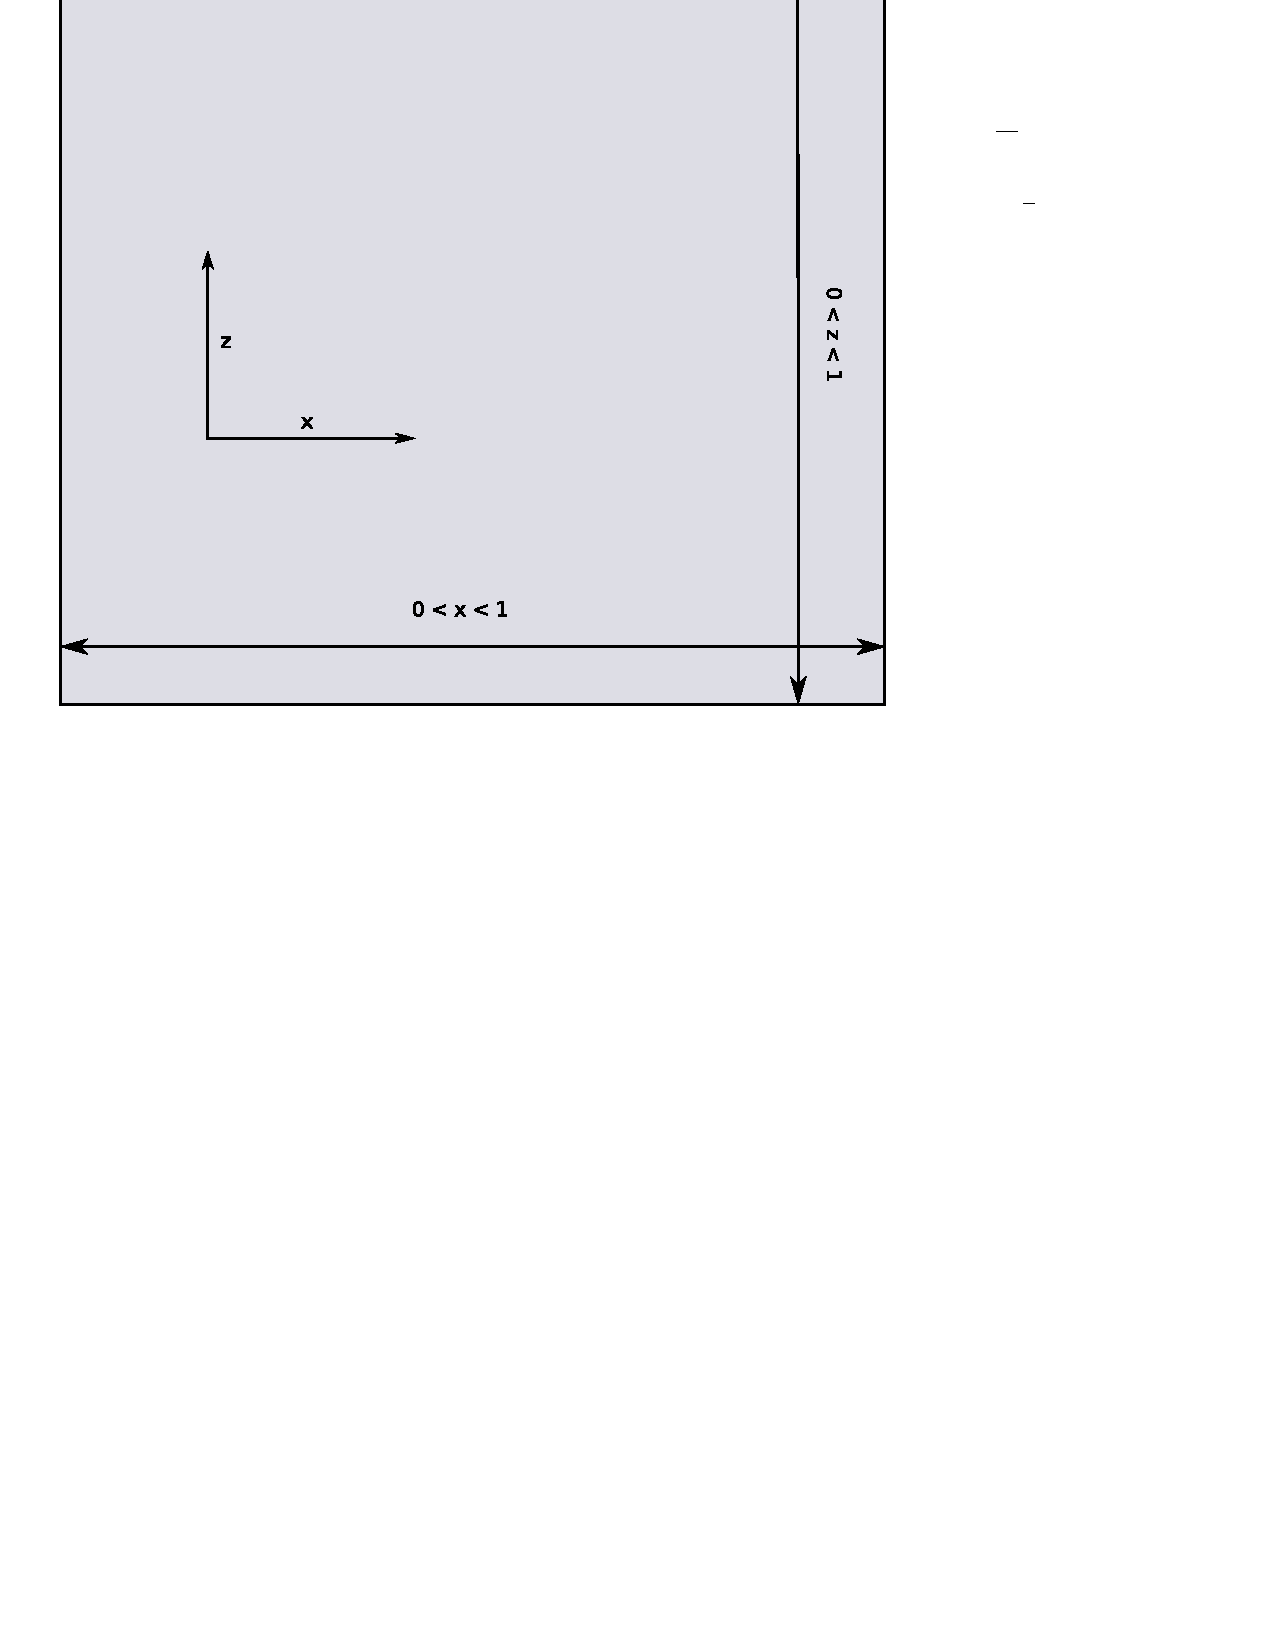
\includegraphics[width=6cm,clip]{../figs/figA}
    \caption[Short caption]{\label{figA} 
      Solution ({\bf SolA}):
      This solution has a box of density $\rho = -\sigma \sin (k_m z) \cos (k_n x)$ .
      It is isoviscous.
      The Boundary conditions are free slip everywhere on the surfaces of the unit box.}
  \end{SCfigure} 
  \vspace{-47mm}
  {\small
  \[
    \hspace{-77mm} \rho = -\sigma \sin (k_m z) \cos (k_n x)
  \]
  }
  \vspace{47mm}
  

